\section{Evaluation} \label{eval}
In this section, we evaluate the performance of \sys based on the RDMA test tools and real applications. We expect to answer the following questions:

\begin{itemize}
\item How about the performance of \sys compared to that of native RDMA for both VMs and containers?
\item Can \sys be adapted to the real-world RDMA applications in both VMs or containers?
\item How about the scalability of \sys?
\end{itemize}

\subsection{Experiment Methodology}


All experiments are carried out on two servers. The settings mainly include three parts: host server, container and virtual machine. 

Each host server is equipped with 4 Intel Xeon E7-4850 2.40GHz 16-core CPUs and 1 TB RAM. The RNIC used is Mellanox ConnectX-3 56 Gb/sec, which performs RDMA communication under Infiniband.  The operating system is CentOS 7.4.1708 (Linux 3.10.0-693.el7.x86\_64). The RDMA driver installed on the host server is Mellanox OFED 4.4-2.0.7.0~\cite{mlnx-ofed}. To keep the consistence, VMs and containers are built based on the same OS images as host. All VMs are based on QEMU(5.1.50)~\cite{qemu} enabled with KVM~\cite{kvm}. We provide 16 cores and 64 GB memory for each VM. We run containers using Docker~(18.06.1-ce)~\cite{docker} and limit the CPU and memory resources to the same settings as the VM. In addition, all the applications are compiled with GCC/G++ 4.8.5 with the O3 compilation configuration. 


\subsection{Basic Evaluation}

Throughput and latency are the key targets of network performance. RDMA supports two different data transmission modes: one-sided and two-sided. Due to the difference performance between them, we evaluate them respectively.

Based on the RDMA benchmark test tool perftest~\cite{perftest}, we evaluated the performance~(throughput and latency) of native RDMA, hardware virtualization SR-IOV,  software virtualization~(FreeFlow) and \sys in VMs or containers. We don't compared the performance of \sys with that of MasQ because it is not open-sourced. For one-sided write operations, we use ``ib\_write\_bw'' and ``ib\_write\_lat'' commands; for one-sided read operation, we use ``ib\_read\_bw'' and ``ib\_read\_lat'' commands. For two-sided operations~(Send and Recv), we use ``ib\_send\_bw'' and ``ib\_send\_lat'' commands. The specific process is: after the RDMA connection is established between the client and the server, the message bytes are transmitted. The message sizes are from 4B to 1MB. For each message size,  it is evaluated iteratively 1000 times and the average results are used for evaluation.  

\subsubsection{\textbf{Throughput}}
\
\noindent

As the data show in Figure~\ref{fig:write-bw} and Figure~\ref{fig:send-bw}, \sys can achieve comparable throughput compared with SR-IOV and native RDMA. When the message gradually increases, such as reaching 64KB, the throughput of each framework tends to be consistent~(from 2K byte message size). The reason is that the bandwidth of RDMA netwrok is saturated after that. %, and the delay overhead of FreeFlow has been covered by waiting delay in RNIC.

For one-sided mode as the data in Figure~\ref{fig:write-bw} show, the average throughput of \sys VM has only 2.9$\%$ slowdown to that of SR-IOV and 3.8$\%$ slowdown to that of native RDMA. And the average throughput of \sys container has only 2.0$\%$ slowdown to that of native RDMA. For two-sided mode as the data in Figure~\ref{fig:send-bw} show, the average throughput of \sys VM has only 1.1$\%$ slowdown to that of SR-IOV and 1.6$\%$ slowdown to that of native RDMA. And the average throughput of \sys container has only 1.4$\%$ slowdown to that of native RDMA.



\begin{figure}[!ht]
	\centering
	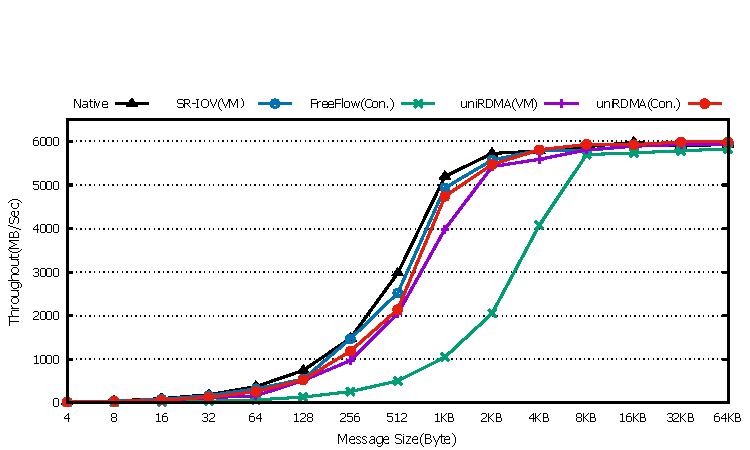
\includegraphics[width=1.0\linewidth]{images/write-bw.pdf}
	\caption{The throughout of one-sided mode.}
	\label{fig:write-bw}
\end{figure}


\begin{figure}[!ht]
	\centering
	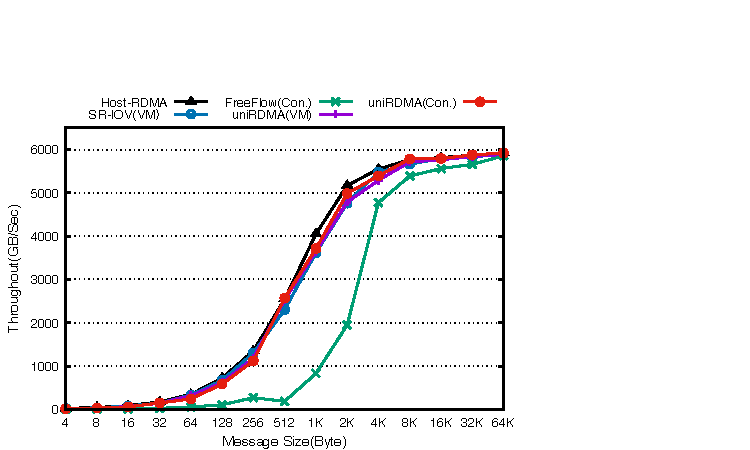
\includegraphics[width=1.0\linewidth]{images/send-bw.pdf}
	\caption{The throughout of two-sided mode.}
	\label{fig:send-bw}
\end{figure}

Compared with FreeFlow, when the message is small, the throughput of \sys has reached 4-6 times that of FreeFlow. Because FreeFlow forwards all data commands to the software virtualization layer for processing. Therefore, the forward latency gradually accumulates and decrease the throughput significantly. However, \sys maps all RDMA resources to execute data commands in the user space of the container or virtual machine. Therefore, there is no latency for commands forwarding in data path.





\subsubsection{\textbf{Latency}}
\
\noindent

The results of two-sided operation are shown in Figure~\ref{fig:send-lat}, and the one of one-sided operation are shown in Figure~\ref{fig:write-lat}. \sys can achieve comparable letency compared with SR-IOV and native RDMA. The latency gradually increases as the forwarding message becomes larger because the main latency has been caused by RNIC data processing.

For one-sided operation, \sys in virtual machine leads to 11\% and 6\% higher latency compared with native RDMA and SR-IOV. The container scenario offers 4\% higher latency than native RDMA. For two-sided operation, the latency of virtual machine is 15\% higher than native RDMA and 5\% higher than SR-IOV. The latency of container is 15\% higher than native RDMA.

Compared with FreeFlow, when the message is small, the latency of \sys has reached 40\% to 60\% of FreeFlow because the overhead of forwarding data path commands to the virtual layer becomes the main latency. \sys removes this problem by removing context switching and copy between virtual instances and the virtual layer.


\begin{figure}[!ht]
	\centering
	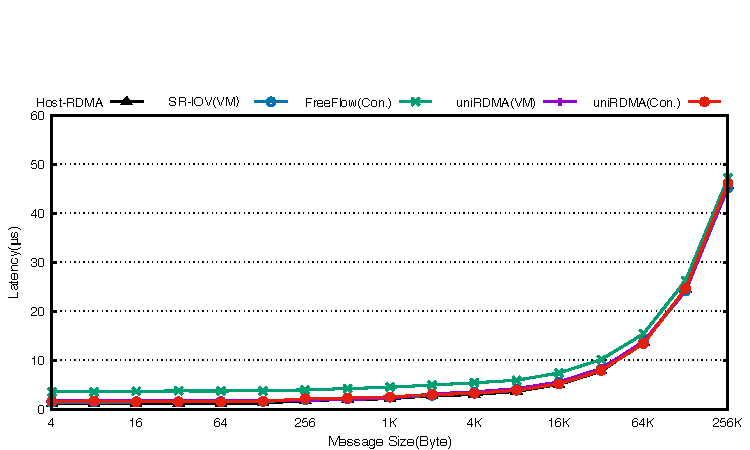
\includegraphics[width=1.0\linewidth]{images/write-lat.pdf}
	\caption{The latencty of one-sided mode.}
	\label{fig:write-lat}
\end{figure}


\begin{figure}[!ht]
	\centering
	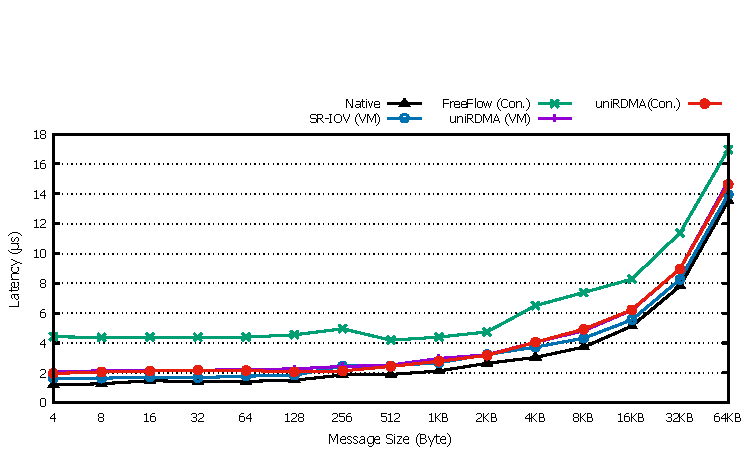
\includegraphics[width=1.0\linewidth]{images/send-lat.pdf}
	\caption{The latencty of two-sided mode.}
	\label{fig:send-lat}
\end{figure}


\subsection{Scalability}

As the applications scalability and servers' hardware capabilities rise, multiple VM and container istances are deployed on a same host. VMs and containers have orders of magnitude far beyond the number of hosts, leaving a great challenge to RDMA virtualization. 

In this paper, we use aggregate throughput, which is the sum of the throughput of multiple parallel RDMA flows at the same time, to measure the scalability of \sys. The thoughput of a individual RDMA flow is fluctating at each moment and the instant RDMA throughput is difficult to align between multiple RDMA flows. Therefore, we collect and summarize the average throughput of each RDMA flow at a certain time segment to obtain the aggregate throughput.

We used one-sided operation (``ib\_write\_bw'' in ~\cite{perftest}) with 2, 4, 8, 16, 32 and 64 virtual instance pairs which send data (65536 Bytes) continuously on two hosts. As shown in Figure~\ref{fig:scabality}, in the VM-only scenario, container-only scenario and hybrid scenario \sys has a good scalability, that is, the throughput in average is reduced by less than 1.4\% when the number of virtual instance pair is up to 64.

The reason that the number of virtual instance pairs is up to 64 is that the maximum support VF for RNIC is 63, that is only up to 63 VMs are supported for RDMA virtualization.

\begin{figure}[!ht]
	\centering
	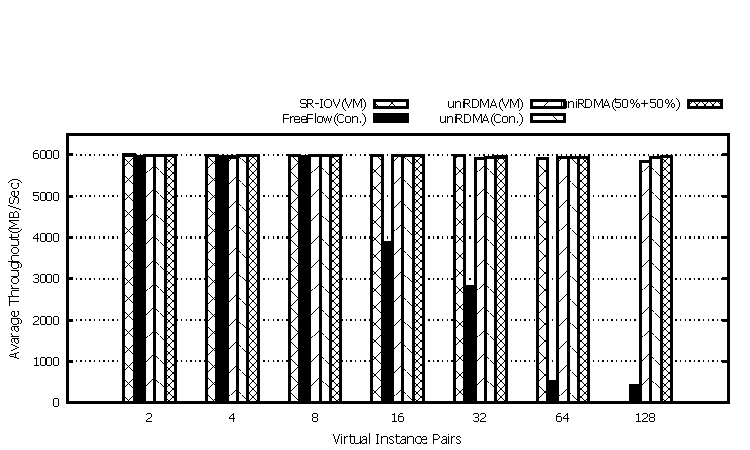
\includegraphics[width=1.0\linewidth]{images/scabality.pdf}
	\caption{Aggregation throughput at different scenarios and scales}
	\label{fig:scabality}
\end{figure}

\subsection{Real-world Applications}

The worth of RDMA is mainly about its optimized performance in real-world applications. RDMA virtualization needs to maintain the performance close to native RDMA. Therefore, we evaluate \sys and other frameworks in a RPC benchmark in radma\_bench\cite{rbench}. In this benchmark, UD transport withe 32-bit immediate header is used between the client and server.

In this paper, the server and client are started on two host servers. The server starts 16 threads, and the client starts 1, 2, 4, 8, 16 threads in turn. This papers separately tested the average throughput of the server in the entire RPC process.

As shown in Figure~\ref{fig:rpc},in the containers, the performance of \sys is approximately same as native RDMA. The
maximum throughput on \sys and native is 11.6 Miops. And in the virtual machines, the performance of \sys is approximately same as the SR-IOV. In total, there is almost no performance loss. Because \sys bypasses the kernel and virtualization layer in the data path, and there is no software forwarding latency caused by virtualization. Even though, in the control path, \sys has a delay because of RDMA Verbs forwarding, this overhead is one-time for the RPC application and it can be ignored. Compared with FreeFlow in the containers, the preformance \sys is better than FreeFlow. Because there is forwarding latency in the data path of FreeFlow.

\begin{figure}[!ht]
	\centering
	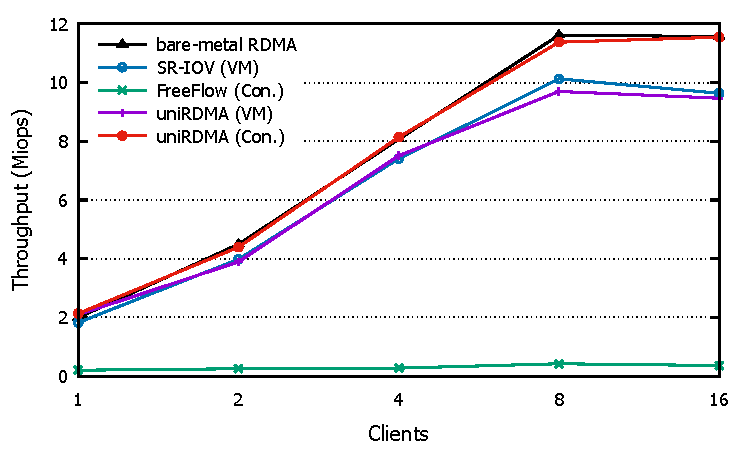
\includegraphics[width=1.0\linewidth]{images/rpc.pdf}
	\caption{The Throughput of RPC}
	\label{fig:rpc}
\end{figure}


